\chapter{Метод нечеткого вывода на основе нечеткого значения истинности}\label{ch:ch2}

\section{Постановка задачи нечеткого вывода}

Лингвистическая модель представляет собой базу правил вида:
\begin{equation}
\label{eqn:fuz-problem-1}
R_k:\ \text{Если}\ x_1\ \text{есть}\ A_{k1}\ \text{и}\ x_2\ \text{есть}\ A_{k2}\ \text{и} \dots \text{и}\ x_n\ \text{есть}\ A_{kn}, \text{то}\ y\ \text{есть}\ B_k,
\end{equation}
где $N$ "--- количество нечетких правил, $A_{ki} \subseteq X_i, i=\overline{1,n}, B_k \subseteq Y$"--- нечеткие множества, которые характеризуются функциями принадлежности $\mu_{A_{ki}}(x_i)$ и $\mu_{B_k}(y)$ соответственно; $x_1, x_2,…,x_n$"--- входные переменные лингвистической модели, причем
\[
[x_1, x_2, ..., x_n]^T = \mathbf{x} \in X_1 \times X_2 \times \dots \times X_n.
\]

Символами  $X_i, i=\overline{1,n}$ и $Y$ обозначаются соответственно пространства входных и выходной переменных. Если ввести обозначения $\mathbf{X}=X_1 \times X_2 \times \dots \times X_n$ и $\mathbf{A_k}=A_{k1}\times A_{k2} \times \dots \times A_{kn}$ , причем
\[
\mu_\mathbf{A_k}(\mathbf{x}) = \underset{i=\overline{1,n}}{T_1} \mu_{A_{ki}}(x_i),
\]
где $T_1$ - произвольная $t$-норма, то правило \ref{eqn:2.1} представляется в виде нечеткой импликации
\begin{equation}
\label{eqn:fuz-problem-2}
R_k: \mathbf{A_k} \to B_k, k=\overline{1,N}.
\end{equation}

Правило $R_k$ можно формализовать как нечеткое отношение, определенное на множестве  $\mathbf{X}\times Y$, т.е. $R_k \subseteq \mathbf{X} \times Y$ - нечеткое множество с функцией принадлежности
\[
\mu_{R_k}(\mathbf{x}, y) = \mu_{\mathbf{A_k} \to B_k} (\mathbf{x}, y).
\]

Модель логического типа определяет задание функции $\mu_{\mathbf{A_k} \to B_k} (\mathbf{x}, y)$ на основе известных функций принадлежности $\mu_{\mathbf{A_k}}(\mathbf{x})$ и $\mu_{B_k}(y)$ с помощью одной из предложенных в [2] функций импликации:
\[
\mu_{\mathbf{A_k} \to B_k} (\mathbf{x}, y) = I(\mu_{\mathbf{A_k}}(\mathbf{x}), \mu_{B_k}(y)),
\]
где $I$"--- некоторая импликация.

Ставится задача определить нечеткий вывод $B'_k \subseteq Y$ для системы, представленной в виде (\ref{eqn:2.1}), если на входах - нечеткие множества.
$\mathbf{A'}=A'_1 \times A'_2 \times \dots \times A'_n \subseteq \mathbf{X}$ или $x_1\ \text{есть}\ A'_1\ \text{и}\ x_2\ \text{есть}\ A'_2\ \text{и} \dots \text{и}\ x_n\ \text{есть}\ A'_n$  с соответствующей функцией принадлежности $\mu_{\mathbf{A'}}(\mathbf{x})$, которая определяется как
\begin{equation}
\label{eqn:fuz-problem-3}
\mu_{\mathbf{A'}}(\mathbf{x}) = \underset{i=\overline{1,n}}{T_3} \mu_{A'_i}(x_i).
\end{equation}

Несинглтонный фаззификатор отображает измеренное $x_i=x'_i, i=\overline{1,n}$ в нечеткое число, для которого $\mu_{A'_i}(x'_i) = 1$ и $\mu_{A'_i}(x_i)$ уменьшается от единицы по мере удаления от  $x'_i$.
В соответствии с обобщенным нечетким правилом modus ponens [2], нечеткое множество $B'_k$ определяется композицией нечеткого множества $\mathbf{A'}$ и отношения $\mathbf{R_k}$, т.е.
\[
B'_k = \mathbf{A'} \circ (\mathbf{A_k} \to B_k),
\]
или, на уровне функций принадлежности
\begin{equation}
\label{eqn:fuz-problem-4}
\mu_{B'_k}(y|\mathbf{x'}) = \sup_{\mathbf{x}\in \mathbf{X}}\left\{\mu_{\mathbf{A'}}(\mathbf{x'})\overset{T_2}{\star} I(\mu_{\mathbf{A_k}}(\mathbf{x}), \mu_{B_k}(y))\right\}.
\end{equation}

В (\ref{eqn:fuz-problem-4}) применена условная нотация, так как ввод в нечеткую систему происходит при определенном значении $\mathbf{x}$, а именно $\mathbf{x'}$. Обозначение $\mu_{B'_k}(y | \mathbf{x'})$ показывает, что $\mu_{B'_k}$ изменяется с каждым значением $\mathbf{x'}$. Вычислительная сложность выражения (\ref{eqn:fuz-problem-4}) составляет $O(|X_1|\cdot |X_2|\cdot \dots \cdot |X_n|\cdot |Y|)$ т.е. экспоненциальная. 

\section{Вывод на основе нечеткого значения истинности}

Используя правило истинностной модификации [1] можно выразить:
\[
\mu_{A'}(\mathbf{x}) = \tau_{A|A'}(\mu_A(x))
\]
где $\tau_{A|A'}$ "--- нечеткое значение истинности (НЗИ) нечеткого множества $A$ относительно $A'$, представляющее собой функцию принадлежности совместимости $CP(A_k, A')$ $A_k$по отношению к $A'$, причем $A'$ рассматривается как достоверное [Дюбуа и др., 1990]:
\[
\tau_{A_k|A'}(v) = \mu_{CP(A_k, A')}(v) = \sup_{\substack{\mu_{A_k}(x) = v \\ x \in X}} \left\{ \mu_{A'}(x)\right\}.
\]

Таким образом НЗИ отражает совместимость факта с посылкой в нечеткой форме. Упрощенные подходы отображают совместимость в одно значение из диапазона впервые представленное в [5].

Перейдем от переменной $x$ к переменной $v$ в выражении нечеткого вывода (\ref{}), обозначив
\[
\mu_{A_k}(x) = v \textrm{ и } \mu_{A'}(x) = \tau_{A_k|A'}(v),
\]
то есть выполним преобразование нечетких множеств на пространстве $X$ в истинностное пространство $[0, 1]$:
\[
?????
\]

Получим:
\begin{equation}
\label{eqn:ftv-compute-4}
\mu_{A'}(x) = \tau_{A_k|A'}(\mu_{A_k}(x)) = \tau_{A_k|A'}(v)
\end{equation}

Тогда (\ref{eqn:fuz-problem-4}) примет вид:
\begin{equation}
\label{eqn:ftv-compute-5}
\mu_{B'_k}(y|\mathbf{x'}) = \sup_{v \in [0,1]}\left\{\tau_{A_k|A'}(v) \overset{T_2}{\star} I(v, \mu_{B_k}(y))\right\}.
\end{equation}

При переходе к нечеткому выводу по $n$ входам формула вычисления НЗИ для нечетких отношений посылки и факта имеет вид:
\begin{equation*}
\tau_{\mathbf{A_k}|\mathbf{A'}}(v) = \sup_{\substack{\mu_{\mathbf{A_k}}(x_1, \dots, x_n) = v \\ (x_1, \dots, x_n) \in \mathbf{x}}} \left\{\mu_{\mathbf{A'}}(x_1, \dots, x_n)\right\} .
\end{equation*}

Или в выражении через операции сверток $t$-норм $T_1$ (\ref{eqn:fuz-problem-2}) и $T_3$ (\ref{eqn:fuz-problem-3}):
\begin{equation}
\label{eqn:ftv-compute-6}
\tau_{\mathbf{A_k}|\mathbf{A'}}(v) = \sup_{\substack{\underset{i=\overline{1,n}}{\mathrm{T_1}}\mu_{A_{ki}}(x_i)=v \\ (x_1, \dots, x_n) \in \mathbf{x}}} \left\{ \underset{i=\overline{1,n}}{\mathrm{T_3}} \mu_{A'_i}(x_i) \right\}.
\end{equation}

Вместо выражения (\ref{eqn:ftv-compute-6}), НЗИ для $n$ входов может быть вычислено как свертка НЗИ по каждому отдельному входу:
\begin{equation}
\label{eqn:ftv-compute-7}
\tau_{\mathbf{A_k}|\mathbf{A'}}(v) = \underset{i=\overline{1,n}}{\mathrm{\tilde{T}}} \tau_{A_{ki}|A'_i}, v \in [0, 1],
\end{equation}
где $\mathrm{\tilde{T}}$ - расширенная по принципу обобщения $n$-местная $t$-норма \cite{kutsenko2015methods}, которая определяется как
\begin{equation}
\underset{i=\overline{1,n}}{\mathrm{\tilde{T}}} \tau_{A_{ki}|A'_i}(v) = \sup_{\substack{\underset{i=\overline{1,n}}{\mathrm{T_1}}v_i = v \\ (v_1, \dots, v_n) \in [0, 1]^n}} \left\{\underset{i=\overline{1,n}}{\mathrm{T_3}}\tau_{A_{ki}|A'_i}(v_i)\right\}
\end{equation}
в результате перехода
\[
\mu_{A_{ki}}(x_i) = v_i \textrm{ и } \mu_{A'_i}(x_i) = \tau_{A_{ki}|A'_i}(v_i).
\]

Тогда для системы с $n$ входами выражения нечеткого вывода на основе НЗИ (\ref{eqn:ftv-compute-5}) примет вид:
\begin{equation}
\label{eqn:ftv-compute-8}
\mu_{B'_k}(y|\mathbf{x'}) = \sup_{v \in [0, 1]} \left\{\tau_{\mathbf{A_k}|\mathbf{A'}}(v) \overset{\mathrm{T_2}}{\star} I(v, \mu_{B_k}(y))\right\}
\end{equation}

Стоит отметить, что выражение (\ref{eqn:ftv-compute-7}) можно записать следующим образом, подчеркнув возможность попарного рекурсивного нахождения свертки НЗИ:
\begin{align*}
\tau_{A_k, A'}(v) & = \underset{i=\overline{1,n}}{\mathrm{\tilde{T}_1}}\tau_{A_{ki}|A'_i}(v_i) \\
& = \left(\dots\left(\left(\mu_{CP(A_{k1}, A'_1)}(v_1)\ \mathrm{\tilde{T}_1}\ \mu_{CP(A_{k2}, A'_2)}(v_2)\right)\ \mathrm{\tilde{T}_1}\ \dots \right) \mathrm{\tilde{T}_1}\ \mu_{CP(A_{kn}, A'_n)}\right).
\end{align*}

Для $n=2$, $\mathrm{\tilde{T}}$ записывается как:
\begin{equation*}
\underset{i=\overline{1,2}}{\mathrm{\tilde{T}}} \tau_{A_{ki}|A'_i}(v) = \sup_{\substack{v_1 \mathrm{ T_1 } v_2 = v \\ v_1, v_2 \in [0, 1]}} \left\{ \tau_{A_{k1}|A'_1}(v_1) \mathrm{ T_3 } \tau_{A_{k2}|A'_2}(v_2) \right\}, v \in [0,1].
\end{equation*}

При вербализации импликации в (\ref{eqn:ftv-compute-8}) она представится в виде:
\begin{equation}
\label{eqn:ftv-compute-9}
\text{Если } \textit{нзи} \text{ есть } \text{ИСТИННО}, \text{ то }\ y\ \text{есть}\ B'_k
\end{equation}

Таким образом, (\ref{eqn:ftv-compute-9}) представляет собой еще одну структуру правил в отличие от канонических структур Заде [10] и Такаги-Сугено [9]. Применение данного правила не зависит от количества входов в нечетких системах.

В формуле (\ref{eqn:ftv-compute-8}) данный подход позволяет переместить процесс вывода в единое пространство НЗИ, где функции истинности, в отличии от различных пространств в подходе Заде, могут быть объединены в более эффективный вычислительный процесс.

\begin{figure}
\label{fig:ftv-schema-comparizon}
\centering
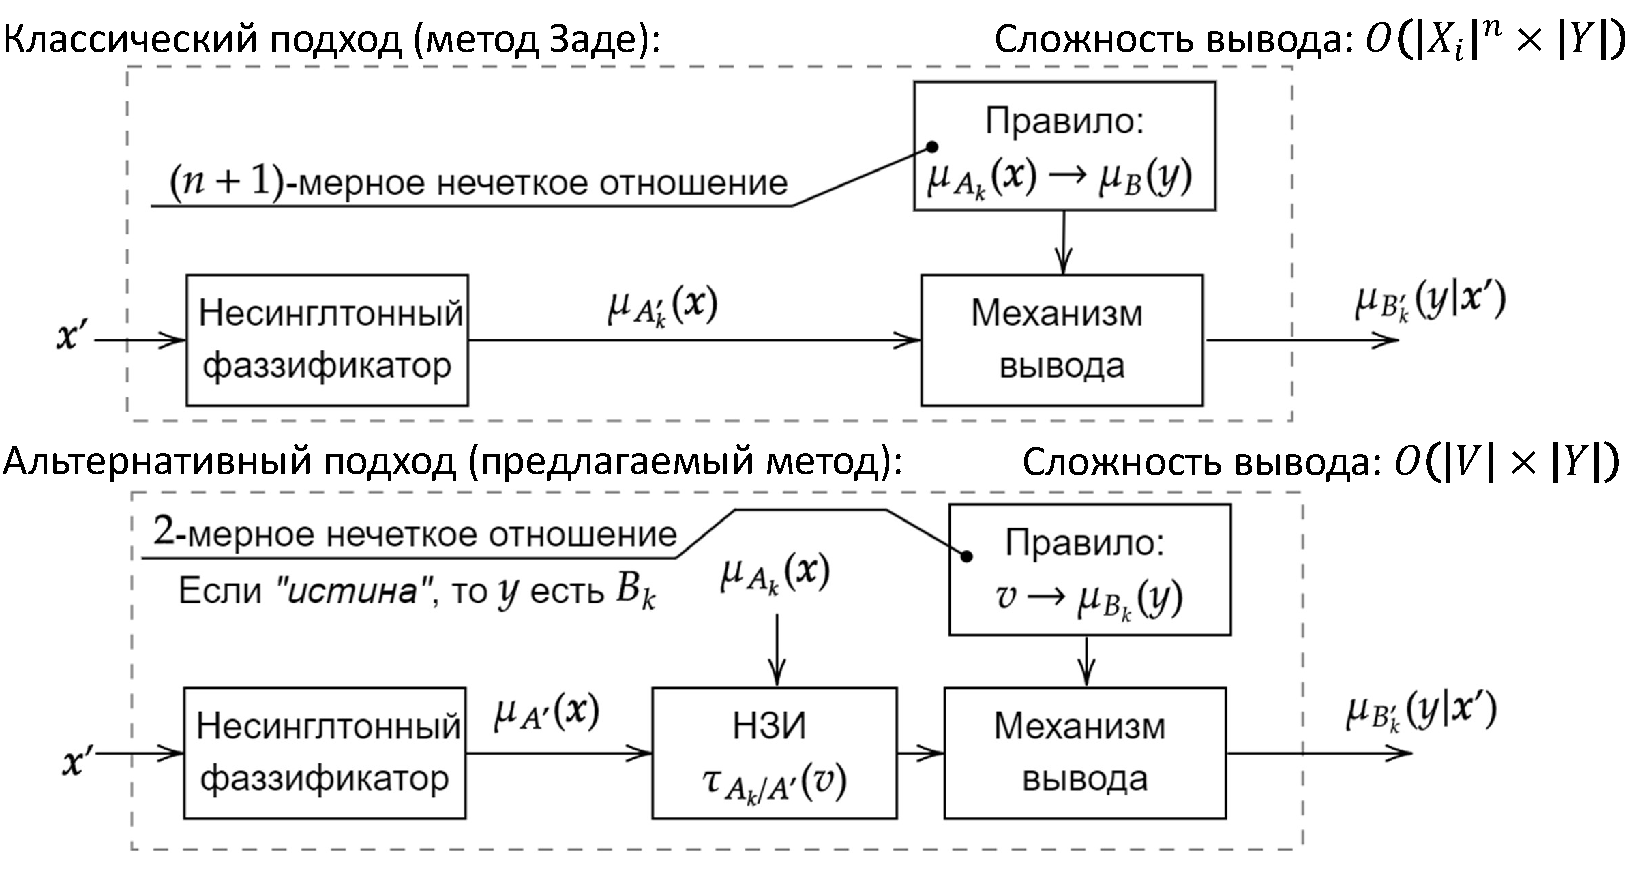
\includegraphics[scale=0.6]{ftv-schema-comparizon}
\caption{Сравнение классической схемы нечеткого вывода и схемы нечеткого вывода на основе НЗИ}
\end{figure}

Порядок функции временной сложности вычисления $B'_k$ на основе выражения (\ref{eqn:ftv-compute-8}) составляет $O\left(n|V|^2+|V|\cdot |Y|\right)$, где $V=CP(A_k, A')$. Сравнение схем нечетких выводов с соответствии с соотношениями (\ref{eqn:fuz-problem-4}) и (\ref{eqn:ftv-compute-8}) представлены на рис. \cref{fig:ftv-schema-comparizon}.

\section{Вывод для систем логического типа}

%Поскольку импликация в формуле (2.4)  не зависит от входных данных (\ref{eqn:2.2}), то предварительно, т.е. до использования композиционного правила (\ref{eqn:2.5}), вычисляется τ_(k,r) (v)=I(v,μ_(B_k ) (y ̅_r )) при k=(1,N) ̅,r=(1,N) ̅, v∈[0,1].



\section{Анализ эффективности методов нечеткого вывода}

\section{Сравнительный анализ логического подхода к нечетком выводу с подходом Мамдани}

Для формирования условий  в которых тот или иной подход к нечеткому выводу показывает  свои сильные стороны имеет смысл провести сравнение.

\section{Сравнение нечеткого вывода с использованием разлчиных методов дефаззификации}

В статье \cite{LEEKWIJCK1999159} описывается подход к сравнению методов дефаззификации.

Описанный метод реализации \cite{eisele1994}.

\subsection{Дефаззификация по методу центра тяжести}

Данный метод можно сопоставить со схемой вычисления математического ожидания случайной величины при данном ее распределении.

\begin{equation*}
y^*_{COG} = \frac{\int_Y y \mu_{B'}(y) dy}{\int_Y \mu_{B'}(y) dy}
\end{equation*}

\subsection{Дефаззификация по методу центра области}

Данный метод можно сопоставить со схемой вычисления медианы случайной величины при заданном ее распределении. Формула вычисления дефаззифицированного значения $y^*_{COA}$ имеет вид:

\begin{equation*}
\int_{\inf Y}^{y^*_{COA}} \mu_{B'}(y) dy = \int_{y^*_{COA}}^{\sup Y} \mu_{B'}(y) dy
\end{equation*}

\subsection{Дефаззификация по методу среднего центра}

\begin{equation*}
y^*_{CA} = \frac{\sum_{k=1}^{N} \bar{y}_k \mu_{B'_k}(\bar{y}_k)}{\sum_{k=1}^{N} \mu_{B'_k}(\bar{y}_k)}
\end{equation*}

\subsection{Дефаззификация по методу суммы центров}

\cite{rutkovskiy2010}

\begin{equation*}
y^*_{COS} = \frac{\int_Y y \sum_{k=1}^{N} \mu_{B'_k}(y) dy}{\int_Y \sum_{k=1}^{N} \mu_{B'_k}(y) dy}
\end{equation*}

\subsection{Дефаззификация по методу среднего максимума}

\begin{equation*}
y^*_{MeOM} = \frac{\sum_{x \in core(B')} x}{|core(B')|},
\end{equation*}
где $core(B') = \left\{y | y \in Y \textrm{ and } \mu_{B'}(y) = \sup_{y' \in Y} \mu_{B'}(y')\right\}$. 

Данный метод аналогичен по схеме вычисления моде случайной величины при заданном ее распределении. В случае унимодального вида функции принадлежности $\mu_{B'}(y)$ данный способ дефаззификации можно упростить до метода максимума функции принадлежности:
\[
y^* = \mathrm{arg\,max}_{y \in Y} \mu_{B'}(y).
\]

\section{Нечеткий вывод при выходной лингвистической переменной с низкой степенью пересечения с функциями принадлежности термов}

Одна из возможностей упрощения процедуры вывода состоит в том, что функции принаждлежностей термов выходной лингвистической переменной достаточно удалены друг от друга и имеют низкую степень взаимного пересечения, то есть выполняется соотношение $\mu_{B_k}(y_r) \approx 0$ при $k \ne r$, что проиллюстрировано на рисунке \cref{fig:out-mf-with-low-crossing}.

\begin{figure}[ht]
	\label{fig:out-mf-with-low-crossing}
	\centering
	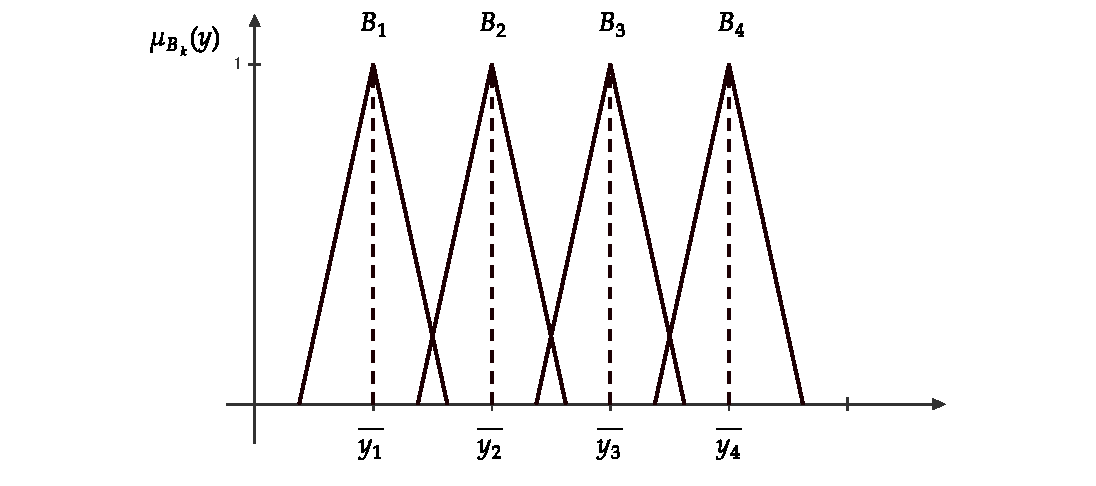
\includegraphics[]{out-mf-with-low-crossing}
	\caption{Пример нечетких множеств, удовлетворяющих условию $\mu_{B_k}(y_r) = 0$ для $y \ne r$}
\end{figure}

Приведенные выклладки справедливы не только для функций принадлежностей отдельных термов, а и для набора кластеризованных в небольшие группы функций принадлжености со значительной степенью пересечения. При такой конфигурации выходного нечеткого пространства нет необходимости вклчать в процесс вывода правила, в которых функции принадлжености консеквента имеют низкий уровень пересечения с ф. п. правил, имеющих высокий уровень срабатывания для данного входа нечеткой системы.

\section{Прогнозирование временных рядов на основе нечетких систем логическогго типа с использованием нечеткого значения истинности}

Для временного ряда $\mathbf{y_t} = (y_1, \dots, y_T)$ величина $y_t$ представляет измеренное значение наблюдаемой переменной в момент времени $t$. Ставится задача предсказания значений $\hat{y}_{t+h}$ для заданного горизонта предсказания $h$.

Модель временного ряда $f(\cdot)$ порядка $p$ использует последние $p$ значений до момента $t$ для оценки значения:
\[
	\hat{y}_{t+h} = f(y_{t-p}, \dots, y_t),
\]
где $p$ - размер лагового окна.

В случае с нечетким прогнозированием временных рядов выполняется фуззификация измеренных значений $(y_1, \dots, y_T)$. Для вычисления параметров функций принадлежности могут использоваться статистические показатели временного ряда, например, дисперсия. В [] для построения фнукций принадлежности используются значение скользящего окна дисперсии. При таком подходе 

Входы нечеткой системы по каждому измерению могут описываться идентичными лингвистическими переменными, заданными на одном базовом множестве и имеющими одинаковую порождающую процедуру для терм-множеств. В [] описаны различные варианты выбора этой порождающей процедуры. Типовые из них:
\begin{itemize}
\item Кластеризация
\end{itemize}

При заданных параметрах лингвистических переменных база правил также может быть построена с использованием различных подходов.

В [] описан подход для одновременного построения базы правил и выделения термов лингвистических переменных на основе многомерной кластеризации с использованием функции схожести класеров 




\FloatBarrier
